\documentclass[letterpaper]{article}
\usepackage{natbib}
\usepackage[utf8]{inputenc}
\usepackage[margin=3.5cm]{geometry}
\usepackage{listings}
\usepackage{adjustbox}
\usepackage{xcolor}
\usepackage{verbatim}
\usepackage{graphicx}%images
\usepackage{fancyhdr}%for headers and footers
\usepackage{adjustbox}
\usepackage{verbatim}
\usepackage{listings}
\usepackage{fancyhdr}
\usepackage{multirow}
\usepackage{amsmath}
\usepackage{array}
\usepackage{mathpazo}
\usepackage{subcaption}
\usepackage{float}
\usepackage{csvsimple}
\usepackage{filecontents}
\usepackage{lscape}
\usepackage{afterpage}
\usepackage{hyperref}
\usepackage{inconsolata}
\usepackage{color}


\newenvironment{conditions}
  {\par\vspace{\abovedisplayskip}\noindent\begin{tabular}
  {>{$}l<{$} @{${}={}$} l}}
  {\end{tabular}\par\vspace{\belowdisplayskip}}


  \newenvironment{conditions_bis}
  {\par\vspace{\abovedisplayskip}\noindent\begin{tabular}
  {>{$}l<{$} @{${}\in{}$} l}}
  {\end{tabular}\par\vspace{\belowdisplayskip}}

\definecolor{pblue}{rgb}{0.13,0.13,1}
\definecolor{pgreen}{rgb}{0,0.5,0}
\definecolor{pred}{rgb}{0.9,0,0}
\definecolor{pgrey}{rgb}{0.46,0.45,0.48}

\lstset{language=Python,
  showspaces=false,
  numbers=left,
  showtabs=false,
  breaklines=true,
  showstringspaces=false,
  breakatwhitespace=true,
  commentstyle=\color{pgreen},
  keywordstyle=\color{pblue},
  stringstyle=\color{pred},
  basicstyle=\ttfamily,
  moredelim=[il][\textcolor{pgrey}]{$ $},
  moredelim=[is][\textcolor{pgrey}]{\%\%}{\%\%}
}



\hypersetup{
    colorlinks,
    citecolor=black,
    filecolor=black,
    linkcolor=black,
    urlcolor=black
}


% ------ HEADERS AND FOOTERS -----------
% \lhead{INFO-F403}
% \rhead{Project Report - Part 1}
%\pagestyle{fancy}
% \rfoot{\thepage}
%\cfoot{}
%\lfoot{Academic Year 2017-18}

\newcommand{\HRule}{\rule{\linewidth}{0.5mm}} %newcommand for cover page

\begin{document}

\begin{titlepage}
\begin{center}


\textsc{\LARGE universit\'e libre de bruxelles}\\[1.0cm]
\textsc{\Large D\'epartment d'Informatique}\\[1.5cm]

% Upper part of the page. The '~' is needed because \\
% only works if a paragraph has started.

\includegraphics[width=0.3\textwidth]{Images/ulblogo.jpg}~\\[1cm]

\textsc{
\large INFO-F404 \\
\Large  Real-Time Operating Systems
 \\[1cm]}
% Title
\HRule \\[0.7cm]

{ \huge \bfseries Project 1 – Audsley  \\[0.7cm] }

\HRule \\[2cm]

% Author and supervisor
\noindent
\begin{center} \large

\emph{Author:}\\
\Large Hakim \textsc{Boulahya}\\
Youcef \textsc{Bouharaoua}
\end{center}
\begin{center} \large

% \emph{Professor:} \\
% Gilles \textsc{Geeraerts}\\

\end{center}

\vfill

% Bottom of the page
{\large \today}

\end{center}
\end{titlepage}

\tableofcontents
\newpage

\section{Feasibility interval}

\paragraph{}

To find the feasibility interval, we implemented a function that finds the least common
multiple of a list of task periods. When this is found, it is just needed to find
the maximum offset to produce the feasibility interval $[O_{max}, O_{max} + 2P]$.
Figure \ref{fig:interval} shows the implementation of the
feasibility interval calculation.

\begin{figure}[H]
    \begin{lstlisting}
def hyper_period(tasks):
    if len(tasks) == 0:
        return None
    elif len(tasks) == 1:
        return tasks[0][T]
    return lcm(*[task[T] for task in tasks])

def interval(tasks_file):
    tasks = parse_tasks(tasks_file)
    omax = max([task[O] for task in tasks])
    P = hyper_period(tasks)
    print(omax, omax + (2 * P))
    \end{lstlisting}
    \caption{Functions of the interval calculation}
    \label{fig:interval}
\end{figure}


\section{Simulator}

\paragraph{Implementation choices}

The simulator of the single FTP simulator is implemented in a discrete manner
from \texttt{start} to \texttt{stop}. For each time steps
we execute functions that will update the
current running job information, the different requests (arrivals or deadlines)
and will store them in data sets. We choose not to print the different
actions during the simulation,
since the simulation is used for other commands such as
the plotter or the audsley algorithm. The output can be produced by
a call to the method \texttt{FTPSimulation.output()}.

\subsection{Periodicity of the requests}

\paragraph{Arrivals periodicity}

The important part of the simulation is to detect the arrivals \textit{i.e.}
the job requests and the deadlines of those jobs. We know that
the job requests for each task are periodic.
Let $\tau_i = (O_i, T_i, D_i, C_i)$ a periodic task. We know that each
job request of $\tau_i$ have a periodicity of $T_i$ with the first request
made at time $O_i$. We can detect if a request for $\tau_i$ occur at time
$t$ using the following formula:

\begin{equation}
  \label{arr_period}
  [(t - O_i) \ge 0] \;\; and \;\; [(t - O_i) \; mod \; T_i = 0]
\end{equation}

The left-side formula is the detection of the first request. If $t - O_i$
is bigger than 0,
then it means that it is possible that $\tau_i$ request a job.
The right-side formula is the detection of a request at time $t$. To detect
which job it is we can make an entire division of $t - O_i$ with
the period $T_i$. Figure \ref{fig:arrival_for} is a excerpt of the arrival
detection.

\begin{figure}[H]
    \begin{lstlisting}
offset, period = self.tasks[task_id][O], self.tasks[task_id][T]
cond = (t - offset >= 0) and ((t - offset) % period) == 0
job_id = (t - offset) // period  # module == 0 i.e. no decimals
return (job_id, True) if cond else (None, False)
    \end{lstlisting}
    \caption{Function of the arrival detection for a task at time $t$}
    \label{fig:arrival_for}
\end{figure}

\paragraph{Deadlines periodicity}

For each job requested job there is a deadline associated \textit{i.e.}
the deadline is also periodic. To detect if a deadline occur at time $t$
of a task $\tau_i$ we can use the same formula (\ref{arr_period}), and
testing the formula a time $t - D_i$. This method actually detect if
a job was requested, and we are a the requested time plus the deadline, the
it is the deadline of this job. Figure \ref{fig:deadline_for} shows
a excerpt of the deadline detection.

\begin{figure}[H]
    \begin{lstlisting}
deadline = self.tasks[task_id][D]
return self.is_arrival_for(t - deadline, task_id)
    \end{lstlisting}

    \caption{Function of the deadline detection for a task at time $t$}
    \label{fig:deadline_for}
\end{figure}


\subsection{Pending jobs}

\paragraph{} To be able to process requested jobs, the simulator uses a list
of list to handle pending jobs. A sublist per task exists. When a request
of a task occurs, the new job is added to the pending jobs sublist of the
task.
The sublists are ordered by task priority. Therefore the job to process
is the first job of the first sublist. If this list is empty, then
it process the first job of the second list, etc. When a job finished its
computation \textit{i.e.} has been processed $C_i$ time, then it is removed
from the pending jobs list. Figure \ref{fig:pending_jobs} shows the snippet
of the function that returns the job to be processed.

\begin{figure}[H]
    \begin{lstlisting}
for sub_jobs in self.pending_jobs:
    for job in sub_jobs:
        return job
return None
    \end{lstlisting}
    \caption{Job to be processed detection}
    \label{fig:pending_jobs}
\end{figure}

\subsection{Events}

\label{sec:events}

\paragraph{}

For each time steps, the simulator stores relevant information that can
be used to output information on the standard output or in a plot.
Those information are stored in an object \texttt{Event}
which is composed of actions that occurs at time $t$:
\begin{itemize}
  \item The job requests
  \item The deadlines (and the missed deadlines)
  \item The computed job
\end{itemize}

\subsection{Hard vs Soft simulation}

\paragraph{}


It is possible to configure the simulation to consider the deadlines as
soft or hard. If the soft configuration is chosen, the simulator will
not stop at deadline misses. If the hard configuration is chosen, the
simulator will stop at the first deadline miss (see section \ref{sec:howto}
to see how to run each configuration).

\subsection{Output}

\paragraph{}


The output production is a post process function. It has been implemented
like this to avoid printing while doing the simulation because the simulation
is used by other part of the project such as the implementation of the
Audsley algorithm or the schedule plotter. The \texttt{output()} method
uses the events of the simulator (section \ref{sec:events}).


\paragraph{}
The simulator provides two approach to the output. The default
mode is the \textbf{request mode}. It provide an output as shown in Figure
\ref{fig:req_mode}. This mode output the requests,
such as arrivals or deadlines, as soon as they occur. So it does output
even if a job is processing during a block.
This mode has been implemented
to provide a more continuous approach to the simulation.

The second approach is the \textbf{preemptive mode}. As explained above
the process block of a job can be divide in multiple blocks if requests
occur during the process. To propose an output that characterise more
the preemptive property of a FTP simulator, the preemptive mode provide
a preemptive results as shown in Figure \ref{fig:pre_mode}.

\paragraph{}
Section \ref{sec:howto} explained how to run the different modes.


\begin{figure}[H]
  \begin{subfigure}{1\textwidth}
    \begin{lstlisting}
    \end{lstlisting}
      \centering
      \begin{lstlisting}[numbers=none]
                              0 5 10 5
                              0 3 20 2
      \end{lstlisting}
      \caption{Tasks set to output $(O_i, T_i, D_i, C_i)$}
  \end{subfigure}
  \begin{subfigure}{.5\textwidth}
      \centering
      \begin{lstlisting}[numbers=none]
      0: Arrival of job T1J1
      0: Arrival of job T2J1
      0-3: T1J1
      3: Arrival of job T2J2
      3-5: T1J1
      \end{lstlisting}
      \caption{Requests mode output}
      \label{fig:req_mode}
  \end{subfigure}
  \begin{subfigure}{.5\textwidth}
      \centering
      \begin{lstlisting}[numbers=none]
      0: Arrival of job T1J1
      0: Arrival of job T2J1
      0-5: T1J1
      3: Arrival of job T2J2
      \end{lstlisting}
      \caption{Preemptive mode output}
      \label{fig:pre_mode}
  \end{subfigure}
\end{figure}

\subsection{Schedule plotter}

The plotter is implemented in the simulation. After running the simulation
the method \texttt{FTPSimulation.plot()} will produce a file
\textbf{scheduler.png}, with the result of the simulation. The computed jobs
data that are gathered during the simulation are used to plot the result.
Figure \ref{fig:plotter} shows example of plots.

\begin{figure}[H]
    \begin{subfigure}{.5\textwidth}
    \centering
    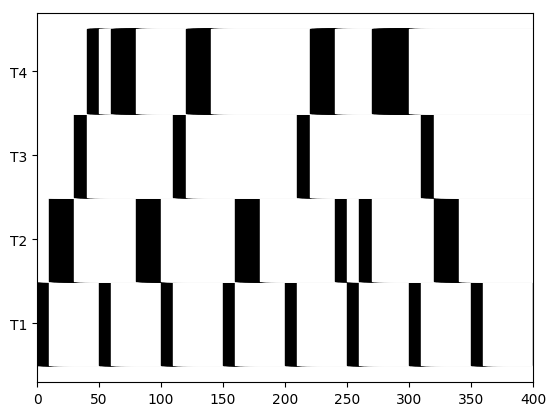
\includegraphics[scale=0.5]{Images/tasks.png}
    \caption{Plot of tasks.txt}
    \end{subfigure}
    \begin{subfigure}{.5\textwidth}
    \centering
    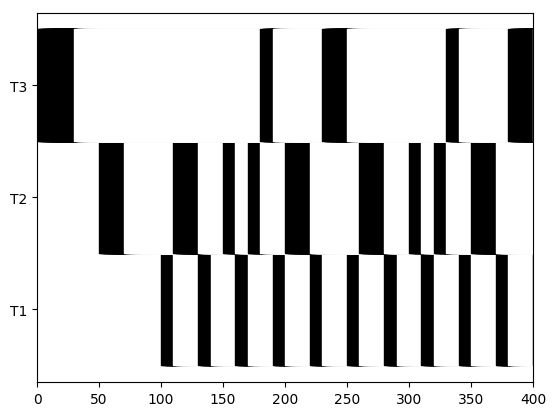
\includegraphics[scale=0.5]{Images/audsley.png}
    \caption{Plot of audsley.txt}
    \end{subfigure}
    \caption{Plot examples}
     \label{fig:plotter}

\end{figure}

\section{Lowest-priority viable}

A task $\tau_{i}$ is lowest priority viable
if and only if and only if all his jobs respect the deadlines when :
\begin{enumerate}
    \item $\tau_{i}$ has the lowest priority
    \item The others tasks has a higher priority
    (the order of thus ones does not influence $\tau_{i}$)
    \item The schedule continues until completion
    (soft deadlines) $\forall \tau_{j}$
\end{enumerate}

Following this definition, the algorithm $lowest-priority-viable$
which takes a list of tasks an id and an interval in parameters,
 check if the id of task given on parameter is LVP by:

\begin{itemize}
    \item Putting the task with given id at the tail of the list
    (to respect the first point of the definition)
    \item Ruining a soft simulation and check if $\tau_{i}$
    missed a job without worrying about the other tasks
    (which respects the second part of the definition)
\end{itemize}
And to do this we have a list of integers which represent
the number of missed jobs for every task when the simulation is running.

\section{Audsley algorithm}

\paragraph{}

The classic Audsley algorithm determines a lowest priority viable
task in the sub-set $\delta \{\tau_{i}$ of $n-1$ tasks
(i.e., assigning priority level $n-1$). The priority assignment
of the Audsley algorithm may leads to a scheduled system
(i.e., priority assignment succeed). But in this project
we were asked to implement a variant of this algorithm
that finds all scheduled system for a given set of tasks.
The excerpt in Figure \ref{fig:audsley_search} shows the implementation of
the variant algorithm.

\begin{figure}[H]
    \begin{lstlisting}
def audsley_search(first, last, tasks, includes, level=0):
    for task_id in includes:
        sub_tasks, sub_task_id = filter_tasks_list(tasks, task_id, includes)
        if lowest_priority_viable(sub_tasks, sub_task_id, first, last):
            print((" " * level) + "Task \%d is lowest priority viable"
                  \% (task_id + 1))
            new_indices = includes[:]
            new_indices.remove(task_id)
            audsley_search(first, last, tasks, new_indices,
                           level + 1)
        else:
            print((" " * level) + "Task \%d is not lowest priority viable"
                  \% (task_id + 1))
    \end{lstlisting}
    \caption{Audsley search algorithm}
    \label{fig:audsley_search}
\end{figure}


The variable level represents the level
of the recursion and the procedure takes a list of all tasks and another
one without the LVP task, the algorithm will print the tasks by levels of
recursion too as explained in the statement of the project.
Figure \ref{fig:audsley_results} shows an example of output that the function
produce.

\begin{figure}[H]

    \begin{subfigure}{1\textwidth}
        \centering
        \begin{tabular}{c c c c}
         $O_i$ & $T_i$ & $D_i$ & $C_i$  \\
        \hline
        100 & 30 & 20 & 10 \\
        50 & 50 & 50 & 20 \\
        0 & 150 & 100 & 30 \\
        \end{tabular}
        \caption{Tasks set}
    \end{subfigure}
    \begin{subfigure}{1\textwidth}

        \begin{lstlisting}[numbers=none,language=bash]
                Task 1 is not lowest priority viable
                Task 2 is lowest priority viable
                 Task 1 is not lowest priority viable
                 Task 3 is lowest priority viable
                  Task 1 is lowest priority viable
                Task 3 is not lowest priority viable
        \end{lstlisting}
        \caption{Output of \texttt{audsley\_search} function}
    \end{subfigure}
    \caption{Audsley results}
    \label{fig:audsley_results}
\end{figure}


\section{Generator}

We were asked to implement a generator of periodic, asynchronous
systems with constrained deadlines based on two parameters
(the utilisation factor and a  number of tasks to generate),
the class \textit{Generator} using the generation method \textit{generate}
produce the set of tasks. The function create tasks, then checks if this
set has the utilisation required if it's the case this set is returned,
if not another random set of tasks is created. For a coherent system
the parameters of every task must respect this inequality:

\begin{equation*}
C_{i} \leq D_{i} \leq T_{i}
\end{equation*}



where, $\forall$  $task_{i}$ :

\begin{conditions}
\hspace{2cm}   C_{i}   &  worst case execution time (WCET)  \\
\hspace{2cm}    D_{i}  &  deadline   \\
\hspace{2cm}    T_{i} &  represents the period
\end{conditions}

knowing that the task utilisation and the system utilisation are respectively:

\begin{equation*}
    U(\tau_{i}) = C_{i} / T_{i}
\end{equation*}


\begin{equation*}
U(\tau) = \sum_{\tau_{i} \in \tau} U(\tau_{i})
\end{equation*}

Remark: utilisation of the generated system
does not have to be equal to the given percentage
but should be very close to it. so the result respects this inequality:

\begin{equation*}
U(\tau)_{given} - 2 \leq U(\tau)_{founded} < U(\tau)_{given}
\end{equation*}



Therefore from what was explain above the randomness
of the parameters of every task follow this logic:


\begin{conditions_bis}
\hspace{2cm}   O_{i}   & [0,300]
The maximum value of the offset were arbitrarily fixed to 300).  \\
\hspace{2cm}   T_{i}     & [1,100]
(The maximum value of the period were arbitrarily fixed to 100).   \\
\hspace{2cm}    C_{i} &  [1,$T_{i}$] \\
\hspace{2cm}    D_{i} &  [$C_{i}$,$T_{i}$]
\end{conditions_bis}


\section{Difficulties}

\paragraph{}

Except for the simulation there were no real difficulties. It is obvious since
most of the part of the project are based on the simulation such as the audsley
algorithm that uses the simulation to determine the lowest priority of tasks.

\paragraph{}

About the periodicity of the simulation,
There were two possible implementation to simulate the scheduler in a
interval given as a parameter. The first idea was to simulate the scheduler
between the feasibility interval $[0, S_n + P)$, but it would be tedious
to do it like this, since we would have to find the corresponding interval
in $[0, S_n + P)$ of the $[start, stop)$ interval of the simulation.
The second possibility is to use the periodicity of the tasks to determine
the requests and deadlines of jobs at a specific time step. For simplicity
of implementation and understanding
we chose the second idea.

\paragraph{}

About audsley algorithm, the real difficulty was actually a way to determine
the lowest priority viable of a specific task with the corresponding set.
To do so we just implemented in the simulation a way to continue the
simulation if when there is a missed deadline. This way it is possible
to detect if a task is LVP only by checking during the simulation if this task
had missed deadlines. The audsley algorithm itself was obvious to implement
since it is just running recursively the LVP checks.

\section{How to run}

\label{sec:howto}

The project is implemented in \texttt{python3}.

\paragraph{Graphical library}

The library used for the graphical part (the plotter) is \textbf{matplotlib}.
To install it run (need root permission):

\begin{lstlisting}[numbers=none]
$ pip install matplotlib
# or
$ pip3 install matplotlib
\end{lstlisting}

To install the library locally, the best way is to use a virtualenv:

\begin{lstlisting}[numbers=none]
$ .local/bin/virtualenv rtosp1
$ source rtosp1/bin/activate
$ pip install matplotlib
\end{lstlisting}

Then switch to the project directory and run the project.

\paragraph{Commands}

The different commands to run the project are listed below, with the additional
arguments:
\begin{lstlisting}[numbers=none]
$ python3 project.py interval [-h] tasks_file
$ python3 project.py sim [-h] [--preemptive] [--hard] start stop tasks_file
$ python3 project.py plot [-h] start stop tasks_file
$ python3 project.py audsley [-h] first last tasks_file
$ python3 project.py gen [-h] number_of_tasks utilisation_factor tasks_file
\end{lstlisting}

\end{document}
